% !TEX encoding = UTF-8 Unicode
\documentclass[fleqn,twoside]{article}
\usepackage[ngerman]{babel}
\usepackage[utf8]{inputenc}
\usepackage[T1]{fontenc}
\usepackage{amsmath}
\usepackage{amssymb}
\usepackage{array}
\usepackage{booktabs}
\usepackage{calligra}
\usepackage{cite}
\usepackage{comment}
\usepackage{csquotes}
\usepackage{enumitem}
\usepackage{eurosym}
\usepackage{fancyhdr}
\usepackage{fdsymbol}
\usepackage{float}
\usepackage{graphicx}
\usepackage{graphicx}
\usepackage{multirow}
\usepackage{nicefrac}
\usepackage{pdfpages}
\usepackage{pifont}
\usepackage{romanbar}
\usepackage{siunitx}
\usepackage{stanli}
\usepackage{tabto}
\usepackage{tabularx}
\usepackage{textcomp}
\usepackage{tikz}
\usepackage{titlesec}
\usepackage{todonotes}
\usepackage{wasysym}
\usepackage{wrapfig}
\usepackage{yfonts}


%Befehle abändern
%Itemize ohne Lücken
\setlist[itemize]{noitemsep, topsep=2pt}
\raggedbottom
%\renewcommand{\todo}[1]{\todo[inline]{#1}}


%Betragsfunktion
\newcommand{\abs}[1]{\ensuremath{\left\vert#1\right\vert}}
%Einheitenfunktion
\newcommand{\un}[2]{{\unit[#1]{\color{black!100}[#2]}}}

\usepackage[pdftex, colorlinks, linkcolor=black, frenchlinks]{hyperref}
\usepackage[a4paper , lmargin = {2.5cm} , rmargin = {2cm} , tmargin = {2.5cm} , bmargin = {2.5cm} ]{geometry}
\pagestyle{fancy}

\title{\Huge{\textfrak{Nichtlineare Modellierung von Stabtragwerken}}}
\author{\calligra{Jonas Konrad}}
\date{\textfrak{\today}}

\begin{document}
\parindent 0pt
\fancyhead[L]{Jonas Konrad}
\fancyfoot[L]{\frakfamily J. K.}
\fancyfoot[R]{\frakfamily }
\fancyfoot[C]{\frakfamily Elastizität ist für Studenten mit einen restlichen Funken an Lebensfreude\\Seite \thepage}
\maketitle \thispagestyle{empty}
%\initfamily %Für Initialien
\begin{center}
\textfrak{Diese Formelsammlung wurde im Wintersemester 2022/23 von Jonas Konrad verfasst. \\Kein Anspruch auf Vollständigkeit oder Fehlerfreiheit.\\LaTex Vorlage: github.com/Neowise33}
\end{center}
\tableofcontents
%\listoftodos
\newpage

\section{Grundbegriffe}
\begin{itemize}
    \item Fließgelenk = Art von Verbindung zwischen zwei oder mehreren Stäben oder Trägern, die es ermöglicht, dass sich die beteiligten Teile in Bezug aufeinander bewegen, ohne dass die Verbindung selbst beschädigt wird. Ein Fließgelenk kann zum Beispiel ein Scharnier, ein Kugelgelenk oder ein Gleitlager sein. In der nichtlinearen Stabtheorie ist es wichtig, die Beweglichkeit der Fließgelenke zu berücksichtigen, da sie die Stabilität und die Verformung des Systems beeinflussen können. In diesem Zusammenhang, Fließgelenke sind häufig modelliert als nichtlineare Elemente, die die Deformationen und die Kräfte innerhalb des Systems beeinflussen können.
    \item Proportionale Laststeigerung $P_\nu = \nu \cdot P$ ; $\nu =$ Laststeigerungsfaktor
    \item Bildung kinematischer Ketten führt zur Erhöhung der Traglast
    \item Imperfektionen
        \begin{itemize}
            \item Vorverdrehung: $\psi_0$
            \item Vorverkrümmung: $\omega_0$
        \end{itemize}
    \item Unsicherheitssatz: \\ Jede Belastung, die an einem geometrisch zulässigen System GGW bildet, stellt einen oberen Grenzwert für die Traglast dar. (3.28)
\end{itemize}

\newpage

\section{Querschnittswerte}

    \subsection{Generelle Begriffe}

        \begin{itemize}
            \item Nutzhöhe d: In QS Mittelpunkt Zugflächenspannung bis Mittelpunkt Druckflächenspannung\\
                Beispiel in Rechteck-Querschnitt: $d=\frac{h}{2}$
        \end{itemize}

    \subsection{QS mit homogenen Material}
        Ablaufplan:
        \begin{enumerate}
            \item Schwerpunkt berechnen (um selsbt gewählten Punkt): $\frac{\sum A \cdot z}{\sum A}$
            \item Flächenträgheitsmoment $I_y$ berechnen
            \item $W_{el} = \frac{I_y}{z_{max}}$ ; $z_{max} = $ maximale Abmessung von SWP bis Rand
            \item $M_{el} = W_{el} \cdot f_y$
            \item Flächenhalbierende berechnen: $A_1 = A_2 \rightarrow \Bar{z}_n$ (Lage SWP von OK-QS aus)
            \item statische Nutzhöhe d
                \begin{itemize}
                    \item $d=\Bar{z}_{s1}-\Bar{z}_{s2}$
                        \begin{itemize}
                            \item $\Bar{z}_{s1} = \frac{\sum (\text{Fläche über SWP}  \cdot \text{Abstand bis OK})}{\sum \text{Flächen über SWP}}$
                            \item $\Bar{z}_{s2} = \frac{\sum (\text{(Fläche unter SWP)}  \cdot \text{(Abstand bis OK)})}{\sum \text{Flächen unter SWP}}$
                        \end{itemize}
                \end{itemize}
            \item $F_D = A_{1 \text{(Fläche bis SWP)}} \cdot f_y$
            \item $M_{pl} = F_D \cdot d$
            \item $W_{pl} = \frac{M_{pl}}{f_y}$
            \item $\alpha_{pl} = \frac{W_{pl}}{W_{el}}$
        \end{enumerate}

    \subsection{Heterogenes Material}
    \begin{minipage}{0.80\textwidth}
        \begin{enumerate}
            \item An logisch gewählten Punkt 1. Maximalspannung des Materials anzeichnen 
            \item Maximale Spannung bis Ränder erweitern (elastisches Modell)
            \item $M_{el} = \sum(\text{Spannung} \cdot \text{Fläche} \cdot \text{Abstand}_{\text{FlächenSWP}} )$
                \begin{itemize}
                    \item Abstand Trapez von SWP = \\ Distanz SWP bis Trapez + $\frac{0,5 \cdot \text{Rechteckfläche} + \frac{2}{3} \cdot \text{Dreieck} / 2}{\text{Min}_{\text{Trapez}}+\text{Max}_{\text{Trapez}} / 2}$
                \end{itemize}
            \item $M_{pl}:$\\
                    \begin{tabular}{cccc|c|}
                        \hline
                        \multicolumn{1}{|c|}{$A_i$} & \multicolumn{1}{c|}{$f_{yd}$} & \multicolumn{1}{c|}{$F_i = A_i \cdot f_{yd}$} & $z_i$ & $M_i = F_i \cdot z_i$ \\ \hline
                        \multicolumn{1}{|c|}{...}   & \multicolumn{1}{c|}{...}      & \multicolumn{1}{c|}{...}                      & ...   & ...                   \\ \hline
                                                    &                               &                                               &       & $\sum = M_{pl}$       \\ \cline{5-5} 
                    \end{tabular}
                \begin{itemize}
                    \item $z_i$ = Abstand SWP von $z_n$
                    \item $\alpha_{pl} = \frac{M_{pl}}{M_{el}}$
                \end{itemize}
                
        \end{enumerate}
    \end{minipage}		
    \begin{minipage}{0.20\textwidth}
        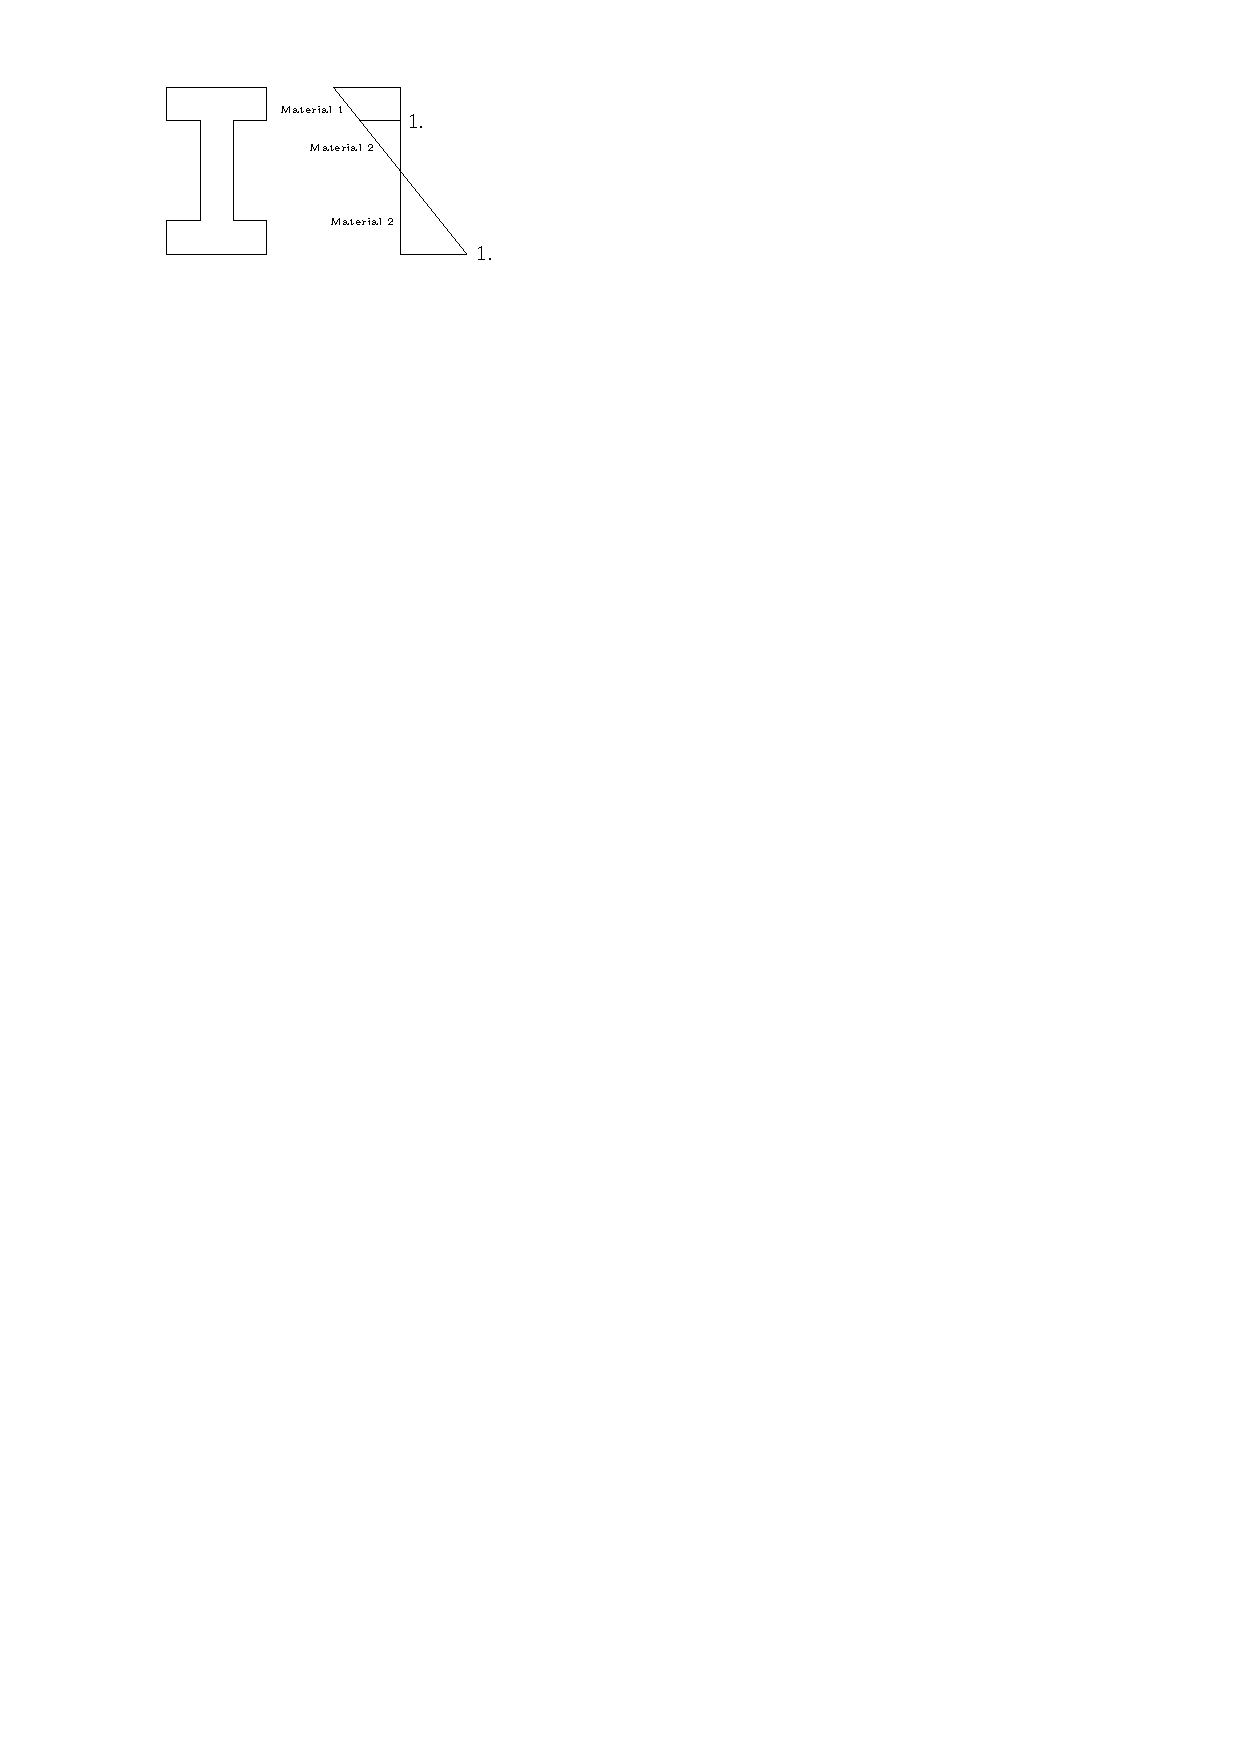
\includegraphics[scale = 0.7]{Grafiken/QS-Werte heterogen.pdf}
    \end{minipage}

    \subsection{Zusätzliche Normalkraft}
        \begin{itemize}
            \item $A_n = \frac{N}{f_y}$: von Fläche ausgehend von Mittelpunkt abziehen
            \item Berechnung über statisches Moment:
                \begin{itemize}
                    \item $A_{erf} = \frac{N}{f_{yd}}$
                    \item $S_{y,neu} = S_{y,QS} - \frac{A_{erf}}{2} \cdot 2 \cdot \frac{A_{erf}}{4} \hateq S_{y,QS} - A_i \cdot z_{si} $ 
                    \item $W_pl = 2 \cdot S_{y,neu}$
                    \item $M_{pl} = W_{pl} \cdot f_{yd}$
                \end{itemize}
        \end{itemize}


\section{Traglastfunktion (Ermittlung $\nu_T$)}

    \subsection{Voruntersuchung}

        \begin{itemize}
            \item statische Unbestimmtheit: $n = a + 3(p-k)-r$
                \begin{itemize}
                    \item a = Auflagerreaktion
                    \item p = Anzahl Stabelemente
                    \item k = Knotenanzahl \\ (alle Knotenpunkte, inkl. Auflager, Gelenke etc. auch feste Rahmenecken, keine freien Stabenden)
                    \item r = Anzahl Stäbe pro Knotenpunkte -1 (nur Gelenkknoten)
                \end{itemize}

            \item Maximale Anzahl Fließgelenke bis kinematische Kette:\\
            n+1 $\rightarrow$ an Einspannungen, Rahmenecken, Einzellasten $\Rightarrow$ dort statische Unbestimmtheit wählen
        \end{itemize}

    \subsection{Ablauf Traglastverfahren}

        \begin{enumerate}
            \item n Gelenke in System einbringen, an Stellen wo wahrscheinlich plastifiziert \\ $\rightarrow$ System stat. bestimmt machen
            \item System zeichnen und Momentenverlauf auftragen:
                \begin{itemize}
                    \item Nullzustand
                    \item Einszustand $(x_1, x_2, x_3,\ldots)$
                \end{itemize}
            \item Überlagerungen (4.36 + 4.38): \\
                $\delta_{10}, \delta_{20}, \delta_{30}, \delta_{11}, \delta_{22}, \delta_{33}, \delta_{12}, \delta_{13}, \delta_{23}$ ; $\delta_{23} \hateq \delta_{32}$  \\
                $\nu = \int_x \frac{\Bar{M} \cdot M}{EI} dx$
            \item Elastizitätsgleichung:\\
                \begin{minipage}{0.50\textwidth}
                    $ \begin{bmatrix} \delta_{11} & \delta_{12} & \delta_{13} \\  & \delta_{22} & \delta_{23} \\ sym &  & \delta_{33} \end{bmatrix}  
                    \cdot
                    \begin{bmatrix} x_1 \\ x_2 \\ x_3 \end{bmatrix}
                    =
                    \begin{bmatrix} \delta_{10} \\ \delta_{20} \\ \delta_{30} \end{bmatrix}
                    \rightarrow x = \begin{bmatrix} \ldots \\ \ldots \\ \ldots \end{bmatrix}$
                \end{minipage}
                \begin{minipage}{0.50\textwidth}
                    $\hateq$ Momente an eingefügten Momentengelenken, quasi Faktor zum überlagern Momentenverläufe\\
                Bei letzten Lastschritt: $x_1 = - \frac{\delta_{10}}{\delta_{11}}$
                \end{minipage}
                 
            \item Momentenverlauf zeichnen
                \begin{enumerate}
                    \item Maximalmomentenauslastung zu 100\% skalieren und einzeichnen (oder Feder entfernen) $\rightarrow \nu_1$
                    \item Falls sich gewählte Momentenfigur nicht ändert 
                        \begin{enumerate}
                            \item Zeile mit ehemals maximalen x aus der Gleichung streichen
                            \item $ x= \begin{bmatrix} \ldots \\ \ldots \end{bmatrix}$
                            \item Erneut Schritt 5 bis benötigte Anzahl an Fließgelenken
                            \item $M_{\text{2,Verlauf}} = M_1 + M_2 + \Delta M_3$
                            \item Aufgetragene Laststeigerungsfaktoren werden auf alle x angewandt. 
                            \item Plastifizierende werden entfernt
                        \end{enumerate}
                    \item Falls Fließgelenk an unvorhergesehener Stelle auftritt \\ $\rightarrow$ Erneut bei 1. starten, aber Momente an FG aufgetragen lassen.
                \end{enumerate}
            \item Gesamter Traglastfaktor: $\nu_T = \nu_1 + \Delta \nu_2 + ...$ \\
                Momentenverlauf im Traglastzustand = letzter Momentenverlauf \\
                $\rightarrow M_T = M_1 + \Delta \nu_2 \cdot \Delta M_2 (M_1 = \Delta \nu_1 \cdot M_0 ; M_2 = M_0)$
            \item Verschiebung:
                \begin{itemize}
                    \item System vor Eintreten letztes FG
                    \item $\Bar{1}$-Verschiebung aufbringen $\rightarrow$ $\Bar{M}$
                    \item $\delta_v^n = \int_x \frac{\Bar{M} \cdot M}{EI} dx \rightarrow m$ (n= System Lastfall n)
                \end{itemize}
        \end{enumerate}

    \subsection{Schrittweises Vorgehen}
        \begin{enumerate}
            \item Vorgegeben Lastfall $M_1$ steigern bis 1.FG auftritt
            \item Gelenk einzeichnen $\rightarrow$ Momentenverlauf zeichnen\\
                    $LZ1+LZ2 \rightarrow 2.FG suchen$
            \item So lange wiederholen bis Systemversagen: $n+1$ Fließgelenke
        \end{enumerate}

    \subsection{Verschiebung nach Entlastung} 
        \begin{itemize}
            \item $M_3 = M_{1(\nu_1)}$ ; $\nu_1 = \nu_T$
            \item $\Bar{1}$-Verschiebung an gesuchten Lager aufbringen und mit $M_E$ überlagern (4.36 + 4.38)
        \end{itemize}
        
\section{KKK - Kombination kinematischer Ketten}

    \subsection{Lage der plastischen Gelenke}
        \begin{itemize}
            \item unter Einzellasten
            \item im Bereich von $\abs{\abs{maxM}}$ bei Streckenlast
            \item bei Einspannungen
            \item bei Rahmenknoten
            \item bei Querschnittsschwächungen
        \end{itemize}

    \subsection{Elementarketten}
        \begin{minipage}{0.5\textwidth}
            \begin{itemize}
                \item Pfeile immer gegen Verdrehung einzeichnen
                \item Trick Bestimmung Anzahl Ketten:
                    \begin{itemize}
                        \item $z=FG -$ 'statische Bestimmtheit'
                        \item $FG$ ablesen, nicht brechnen
                    \end{itemize}
                \item Knotenketten: oft biegesteife Knoten
                \item Rahmenketten: ein Stab verschiebt sich
            \end{itemize}
        \end{minipage}
        \begin{minipage}{0.5\textwidth}
            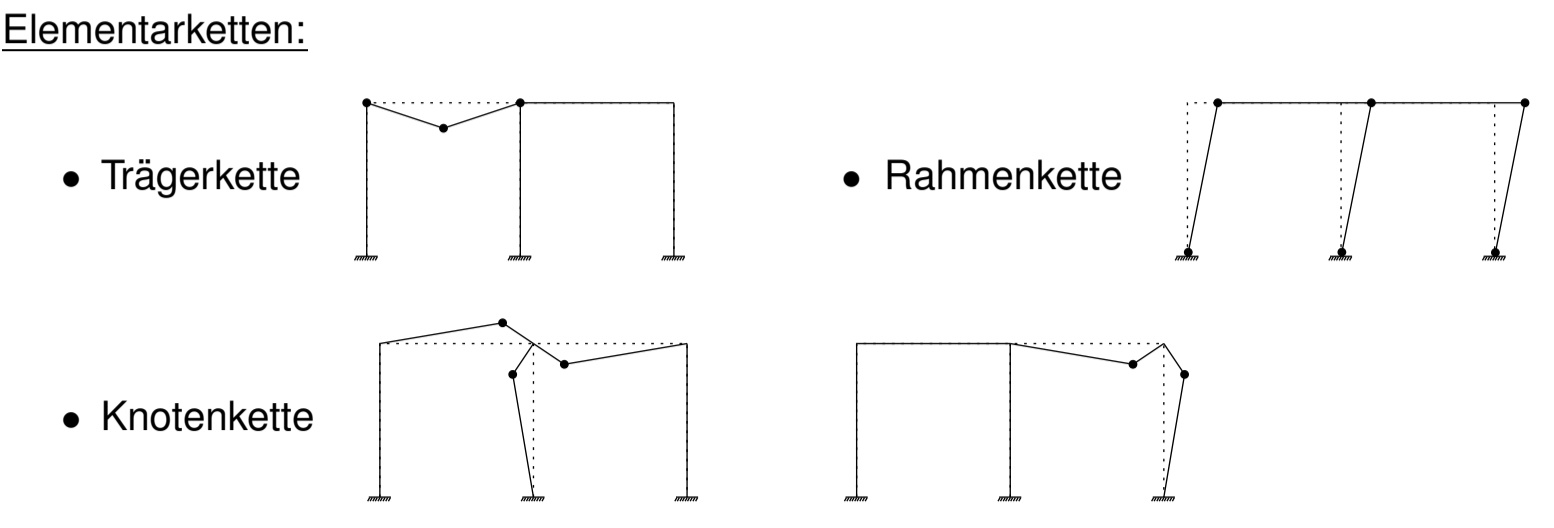
\includegraphics[scale = 0.2]{Grafiken/Elementarketten.png}
        \end{minipage}

        
    \subsection{Ermittlung der plastischen Grenzlast}
        \begin{enumerate}
            \item $r=2\cdot m +m_F - m_G$
                \begin{itemize}
                    \item $r$ = Zahl der möglichen plastischen Gelenke (An biegesteifen Ecken: pro Stab 1)
                    \item $m$ = Anzahl der Grundelemente (alle Stäbe aufteilen wie in RSX)
                    \item $m_F$ = Anzahl im Feld belasteter Elemente
                    \item $m_G$ = Anzahl der an Momentengelenke grenzende Elemente
                \end{itemize}

            \item $z=r-n$
                \begin{itemize}
                    \item $z=$ Anzahl der möglichen Elementarketten
                    \item $r=$ Zahl der möglichen plastischen Gelenke
                    \item $n=$ stat. Unbestimmtheit bzgl. M
                \end{itemize}
            \item Innere \& äußere Arbeit bestimmen:
                \begin{itemize}
                    \item Innere Arbeit: $A_i = \sum \varphi \cdot (\text{Verformungsmomente } M_{pl}) $
                    \item Außere Arbeit: $A_a = \varphi \cdot l \cdot \text{Last} \hateq \text{Moment aus äußerer Last}$ 
                \end{itemize}
            \item Für jede Elementarkette obere Schranke $P_{k i n}$ bestimmen.
            \item Addition von Elementarketten, so dass
                \begin{itemize}  \item Äußere Arbeit $A_a$ möglichst groß \item Innere Arbeit $A_i$ möglichst klein \item $\nu_T=\frac{A_i}{A_a} \rightarrow \min$ \end{itemize}
                Dies ist am besten zu erreichen, wenn sich bei der Kombination der Elementarketten plastische Gelenke wieder aufheben. (Die Kombinationskette darf nur einen Freiheitsgrad aufweisen.)
            \item Kontrolle: $\|M\| \leq M_{p l}$\\
                Damit ist der statische Satz erfüllt und die plastische Grenzlast ist eindeutig bestimmt. Falls $\|M\| \leq M_{p l}$ nicht erfüllt ist, neue Kombinationskette wählen.
            \item Anzahl der möglichen Kombinationen $l=2^z-1$
        \end{enumerate}

    \subsection{Überprüfung ob Traglastzustand}
        \begin{itemize}
            \item Überprüfung ob $\abs{M} \leq M_{pl}$
            \item Ansonsten zusätzlich aufschreiben:
                \begin{itemize}
                    \item Statik: GGW erfüllt $\checkmark$
                    \item Werkstoff: alle $\abs{M} \leq M_{pl}$ $\checkmark$
                    \item Geometrie: siehe Versagensfigur $\checkmark$
                    \item positive Dissipationsenergie $\checkmark$
                \end{itemize}
        \end{itemize}
    \subsection{Tabellarische Kombination kinematische Ketten}
        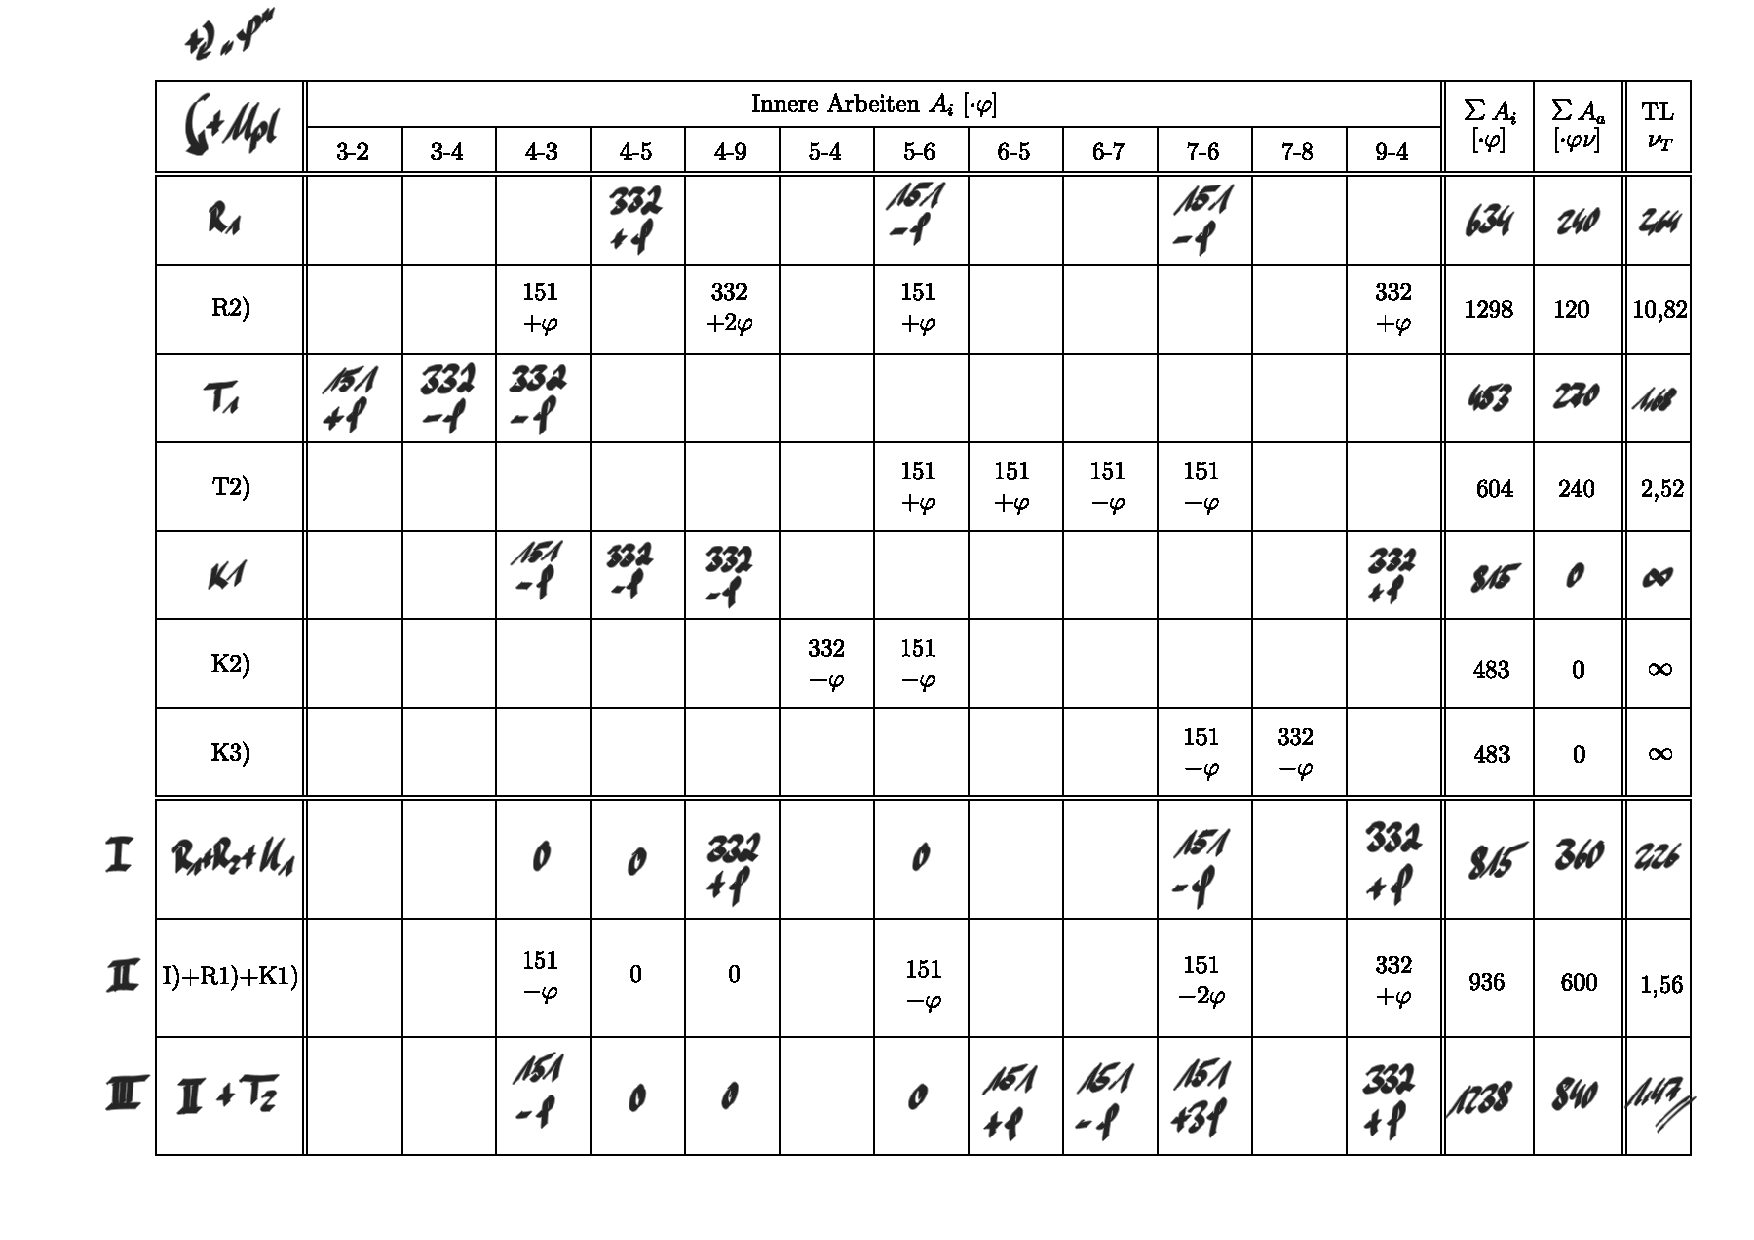
\includegraphics[scale = 0.55]{Grafiken/KombinationElementarketten.pdf}

\section{VV nach Theorie II. Ordnung}
    \begin{itemize}
        \item Stabhennzahl: $\alpha= L \sqrt{S/EI}$
        \item Druchleraffe aud Unoten $\rightarrow$ Knotenvedrehung audbringen
        \item Linienlasten aud Stab $\rightarrow$ Verdrehung an Einspanmang daneben
        \item Einzellasten führen zur Verschicbung des Sustems
        \item Anbringen wo Fliekgelente oder Verschicbungen audtreten honnen Ls stat. Unbestimmtheit+1
        \item Bei komplexeren Verschiebungen die Gelenkfigur zeichnen
    \end{itemize}

    \subsection{Ablauf}
        \begin{enumerate}
            \item Geometrisch bestimmtes Grundsystem aufzeichnen
            \item Nullzustand: Lasten an $r_{1-n}$ berechnen
            \item Lastzustände $r^1=1 ; r^2=1 ; r^3=1 ; \ldots$ anbringen
                \begin{itemize}
                    \item $GGW$ am eingefügte Knoten aufstellen $\rightarrow K_n$ für Knoten
                    \item Eingefügte Lager mit PVV berechnen $\rightarrow K_n$ für Auflager
                    \item Eingefügte Lager mit PVV berechnen $\rightarrow K_n$ für Auflager
                        \begin{itemize}
                            \item Quasi Summe (Kraft $\cdot$ Wirkung) resultierende Vertikal/Horizontalkräfte
                            \item Wirkung zum berechnen z.B. Kraft $r_2$ aus Verschiebungsfigur zu $r_2$
                                \begin{itemize}
                                    \item Querkraft $\cdot$ Verschiebungsfigur
                                    \item Moment $\cdot$ Verdrehung
                                    \item Normalkraft $\cdot$ $\varphi$ $\cdot$ Verschiebung\\
                                        (Verschiebung aus Lastzustand ; $\varphi$ aus Gelenkfigur)
                                    \item Drehfeder: $c_F$ $\cdot$ Verdrehung
                                    \item Wegfeder: $k_F$ $\cdot$ Verschiebung
                                \end{itemize}
                            \item $K$ oder $z$: unbekannte Knotengrößen
                        \end{itemize}
                \end{itemize}
            \item $GGW$ (Bsp.): $\begin{aligned} & U_1=M_2+M_3 \\ & U_2=M_4 \\ & U_3=0\end{aligned}$
            \item $PVV \text{(Bsp.)}: r^4=1: 1 \cdot K_4-\frac{1}{L_1}\left(M_1+M_2\right)$\\
                $\rightarrow$ Auf welche Knoten/Stabkräfte hat Verschiebung Einfluss (für alle eingefügten Auflager durchführen)\\ \\
                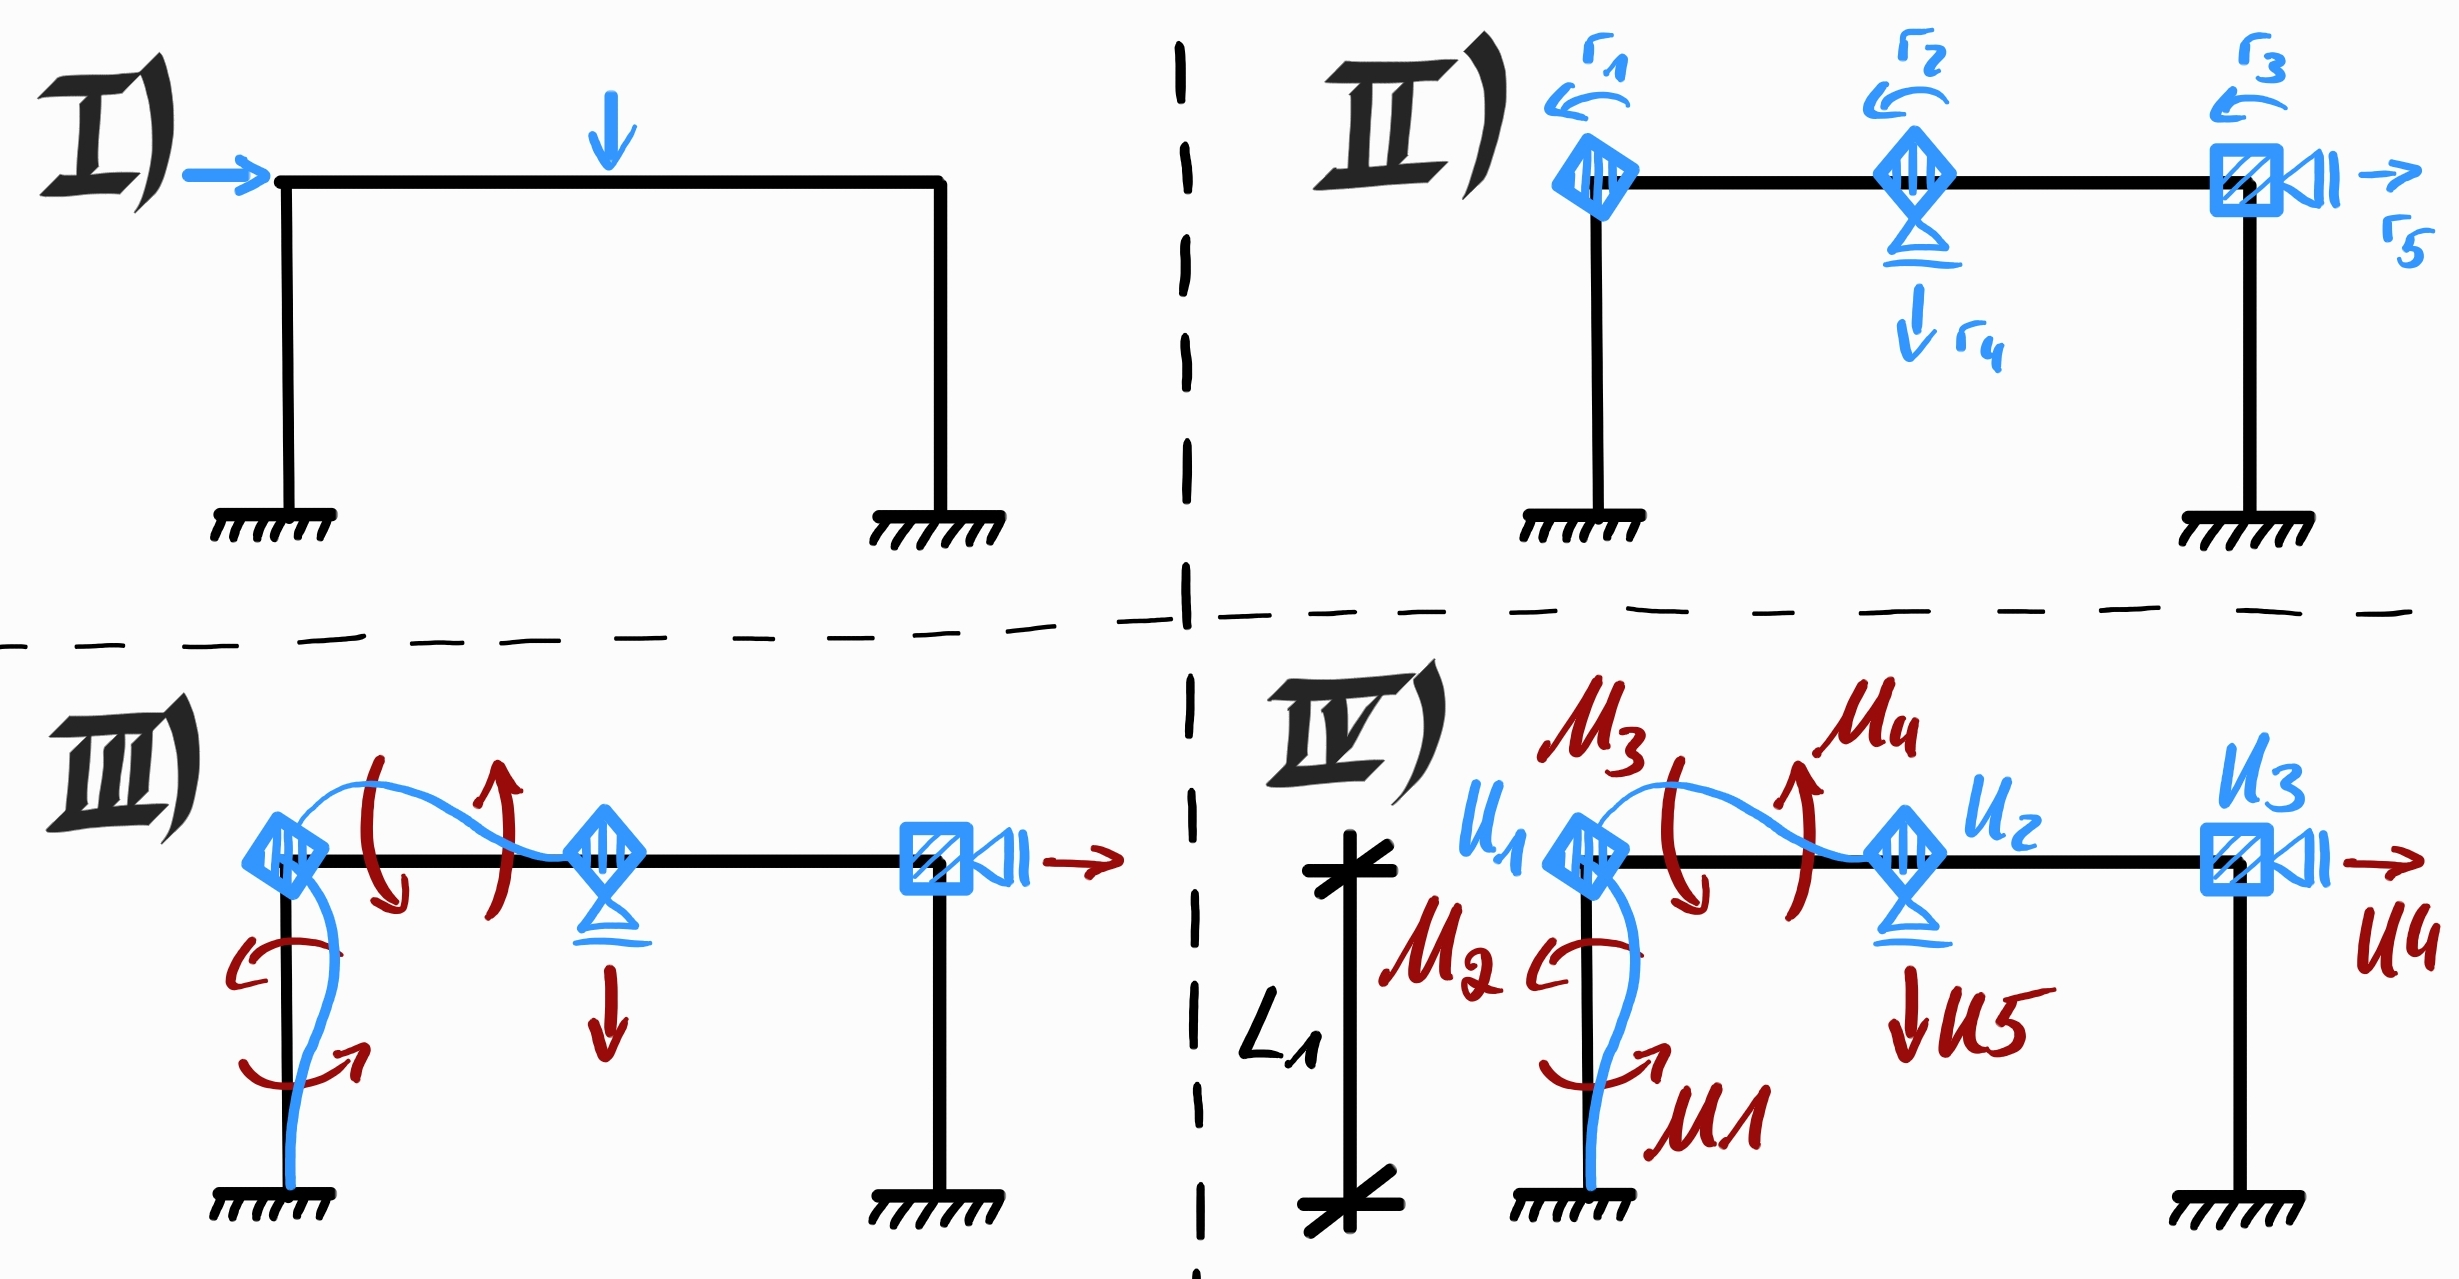
\includegraphics[scale=0.1]{Grafiken/Ablauf VV.jpg}\\
                Zu III): Aus Tafeln für Theorie 1. Ordnung oder Theorie 2. Ordnung\\
                PVV: P-$\Delta$-Effekt nur beachten in Zustand mit tatsächlicher Translation
            %Die nächsten Zeilen sind wirklich hässlich programmiert, aber passt ja zu dem elendigen Fach 
            \item Kompabilitätsbedingungen aufstellen:\vskip 2mm
                $ \begin{smallmatrix} \phantom{r_1} \\\begin{matrix}  K_1 \\ K_2 \\ K_3 \\ K_4 \\ K_5 \end{matrix} \end{smallmatrix}$ 
                $ \begin{smallmatrix} \textrm{ \tiny $r_1=1 \hspace{1.5mm} r_2=1 \hspace{1.5mm} r_3=1 \hspace{1.5mm} \ldots$ \tiny } \\ \begin{bmatrix}  \ldots &  \ldots &  \ldots &  \ldots \\  \ldots &  \ldots &  \ldots &  \ldots  \\  \ldots &  \ldots &  \ldots &  \ldots  \\  \ldots &  \ldots &  \ldots &  \ldots  \\  \ldots &  \ldots &  \ldots &  \ldots \end{bmatrix} \end{smallmatrix}$
                $ \begin{smallmatrix} \phantom{r_1} \\\begin{bmatrix}  r_1 \\ r_2 \\ r_3 \\ r_4 \\ r_5 \end{bmatrix} \end{smallmatrix}$
                $=$
                $ \begin{smallmatrix} \phantom{r_1} \\\begin{bmatrix}  \vdots \\ \vdots \\ z \\ \vdots \\ \vdots\end{bmatrix} \end{smallmatrix}$\\
                $\hspace*{2.15cm} K \hspace*{1.2cm} \cdot \hspace*{0.18cm} r_i \hspace*{0.23cm} = \hspace*{0.2cm} z$ 
                        \begin{itemize} 
                            \item K = Knoten-/Auflagerlasten aus virtuellen Verschiebungen 
                            \item $z = r_1,r_2,r_3,r_4,r_5$ aus Nullzustand
                            \item Negative Normalkraft (Druck) wirkt Steifigkeitsmindernd $\rightarrow$ Wird in Gleichung auf K-Tensor addiert
                        \end{itemize}
           \item Momentenverlauf während Lastschritt n
                \begin{itemize}
                    \item $M = M^{(\text{n-1})} + \sum_k r^i \cdot M^k$\\
                        (Moment im Grundzustand (stat. bestimmt) $+ r_1 \cdot M_1 + r_2 \cdot M_2$)
                    \item $M^k$: Momente an eingefügten Stellen zu $r_1 = 1; r_2 = 1; \ldots$
                \end{itemize}
            \item Fließgelenk einfügen \& $M_{pl}$ antragen
            \item Partiell Kompabilitätsbedingungen ausrechnen
        \end{enumerate}

    \subsection{Entlastung}
        \begin{itemize}
            \item $M_E = M_{1(\nu_1)} $ ; $\nu_1 = \nu_T$
            \item Ersten Momentenverlauf ($M_0$) mit Laststeigerungsfaktor $\nu_T$ abbilden
            \item $M_{\text{verbleibend}} = M_T + M_E$
        \end{itemize}





    
\end{document}